%; whizzy chapter$B!!(B-dvi
% -initex iniptex -latex platex -format platex -bibtex jbibtex -fmt fmt
% $B0J>e(B whizzytex $B$r;HMQ$9$k>l9g$N@_Dj!#(B

%     Tokyo Debian Meeting resources
%     Copyright (C) 2012 Junichi Uekawa
%     Copyright (C) 2011 Nobuhiro Iwamatsu

%     This program is free software; you can redistribute it and/or modify
%     it under the terms of the GNU General Public License as published by
%     the Free Software Foundation; either version 2 of the License, or
%     (at your option) any later version.

%     This program is distributed in the hope that it will be useful,
%     but WITHOUT ANY WARRANTY; without even the implied warranty of
%     MERCHANTABILITY or FITNESS FOR A PARTICULAR PURPOSE.  See the
%     GNU General Public License for more details.

%     You should have received a copy of the GNU General Public License
%     along with this program; if not, write to the Free Software
%     Foundation, Inc., 51 Franklin St, Fifth Floor, Boston, MA  02110-1301 USA

%  preview (shell-command (concat "evince " (replace-regexp-in-string "tex$" "pdf"(buffer-file-name)) "&"))
% $B2hA|%U%!%$%k$r=hM}$9$k$?$a$K$O(Bebb$B$rMxMQ$7$F(Bboundingbox$B$r:n@.!#(B
%(shell-command "cd image201304; ebb *.png")

%%$B$3$3$+$i%X%C%@3+;O!#(B

\documentclass[mingoth,a4paper]{jsarticle}
\usepackage{monthlyreport}

% $BF|IU$rDj5A$9$k!"Kh7nJQ$o$j$^$9!#(B
\newcommand{\debmtgyear}{2013}
\newcommand{\debmtgmonth}{4}
\newcommand{\debmtgdate}{20}
% started from zero:
% (let ((year 2013) (month 4)) (+ (* (- year 2005) 12) month -1))
\newcommand{\debmtgnumber}{99}

\begin{document}

\begin{titlepage}
\thispagestyle{empty}
% $B%?%$%H%k%Z!<%8(B:$BJT=8I,MW$JItJ,$O:G=i$N%^%/%m$KHt$P$9$3$H(B

\vspace*{-2cm}
$BBh(B\debmtgnumber{}$B2s(B $BEl5~%(%j%"(B Debian $BJY6/2q;qNA(B\\
\hspace*{-2cm}

\includegraphics{image2012-natsu/dotdeb.pdf}\\
\hfill{}\debmtgyear{}$BG/(B\debmtgmonth{}$B7n(B\debmtgdate{}$BF|(B

% $B$3$3$O%"%C%W%G!<%H$9$k$3$H(B
% $BA43QJ8;z$K$7$J$$$H%U%)%s%H$N%5%$%:$,9g$o$J$$$N$GCm0U(B
\rotatebox{10}{\fontsize{32}{32} {\gt $BFC=8#1!'(B $B#s#a#m#b#a$GE}9gG'>Z(B}}

\rotatebox{10}{\fontsize{32}{32} {\gt $BFC=8#2!'(B $B3+H/4D6-4IM}(B}}

\vspace*{-2cm}
\hfill{}
\includegraphics[height=6cm]{image200502/openlogo-nd.eps}
\end{titlepage}

\dancersection{Introduction}{$B>e@n(B $B=c0l(B}

\begin{multicols}{2}
 

 $B:#7n$N(BDebian$BJY6/2q$X$h$&$3$=!#$3$l$+$i(BDebian$B$N@$3&$K$"$7$rF'$_F~$l$k$H(B
 $B$$$&J}$b!"$9$G$K$I$C$W$j$H$D$+$C$F$$$k$H$$$&J}$b!"7n$K0l2s(BDebian$B$K$D$$(B
 $B$F8l$j$^$;$s$+!)(B

 Debian$BJY6/2q$NL\E*$O2<5-$G$9!#(B

 \begin{itemize}
 \item \underline{Debian Developer} ($B3+H/<T(B)$B$N0i@.!#(B
 \item $BF|K\8l$G$N!V(B\underline{$B3+H/$K4X$9$k>pJs(B}$B!W$r@0M}$7$F$^$H$a!"%"%C%W%G!<%H$9$k!#(B
 \item \underline{$B>l(B}$B$NDs6!!#(B
 \begin{itemize}
  \item $BIaCJ$P$i$P$i$J>l=j$K$$$k?M!9$,(B face-to-face $B$G=P2q$($k>l$rDs6!(B
	$B$9$k!#(B
  \item Debian $B$N$?$a$K$J$k$3$H$r8l$k>l$rDs6!$9$k!#(B
  \item Debian$B$K$D$$$F8l$k>l$rDs6!$9$k!#(B
 \end{itemize}
 \end{itemize}		

 Debian$B$NJY6/2q$H$$$&$3$H$G5f6KE*$K$O;22C<TA40w$,(BDebian Package$B$r$,$j$,$j(B
 $B$H:n$k%9!<%Q!<%O%C%+!<$K$J$C$?;Q$rLQA[$7$F$$$^$9!#>pJs$N6&M-!&3hMQ$rDL$7(B
 $B$F(B Debian$B$N:#8e$NG=F0E*$JE83+$X$NEZBf$H$7$F!"!V>l!W$H$7$F$N6u4V$rDs6!$9(B
 $B$k$N$,L\E*$G$9!#(B

\end{multicols}

\newpage

\begin{minipage}[b]{0.2\hsize}
 \definecolor{titleback}{gray}{0.9}
 \colorbox{titleback}{\rotatebox{90}{\fontsize{80}{80} {\gt $B%G%S%"%sJY6/2q(B} }}
\end{minipage}
\begin{minipage}[b]{0.8\hsize}
\hrule
\vspace{2mm}
\hrule
\begin{multicols}{2}
\tableofcontents
\end{multicols}
\vspace{2mm}
\hrule
\end{minipage}

\dancersection{$B;vA02]Bj(B}{$B>e@n(B $B=c0l(B}

$B:#2s$N;vA02]Bj$O0J2<$G$9(B:
\begin{enumerate}
 \item $B:G6a(BDebian$B$N%"%+%&%s%H!&%7%9%F%`4IM}$G9M$($F$$$k$3$H(B
 \item Debian$B$G$N3+H/4D6-$r$I$&4IM}$7$F$$$k$+(B
\end{enumerate}
$B$3$N2]Bj$KBP$7$FDs=P$$$?$@$$$?FbMF$O0J2<$G$9!#(B
\begin{multicols}{2}
{\small
 %; whizzy-master ../debianmeetingresume201304.tex
% 以上の設定をしているため、このファイルで M-x whizzytex すると、
% whizzytexが利用できます

\begin{prework}{ べつやく }

\preworksection{最近Debianのアカウント・システム管理で考えていること}

ユーザアカウントの管理について特に意識したことがありません。ログイン時の
 パスワードを共通化できる仕組みがあるらしい・・・ぐらいの認識です。

\end{prework}

\begin{prework}{ koedoyoshida }

\preworksection{最近Debianのアカウント・システム管理で考えていること}

会社のサーバはLinux系で統一されているので、uid,gid,アカウント名をそれに合わせる程度です。
ldap連携も可能ですが、自分の管理しているマシンでは(社内向けのサービスを
 提供していないので)行っていません。

\preworksection{Debianでの開発環境をどう管理しているか}

stable環境にchrootでsid環境を作るorVMware環境上へ構築しています。

\preworksection{SambaをWindowsのドメインに参加させたことはありますか。}

「SambaをWindowsのドメインに参加させたこと」、「Linuxのユーザ認証をWindowsに統合したこと」はありません。
逆にsambaをDCとしてwindowsクライアントを参加させたことはあります。
\end{prework}

\begin{prework}{ ribbon@ns.ribbon.or.jp }

\preworksection{SambaをWindowsのドメインに参加させたことはありますか。}
あります。
\preworksection{参加させたことがある方、ハマったところを教えてください}
バージョンによって挙動が違うところです。
\end{prework}

\begin{prework}{ dictoss(杉本 典充) }

\preworksection{最近Debianのアカウント・システム管理で考えていること}

サーバで使っていても自分しか使用しないので、個人アカウントを作って完
 結してしまっている。

\preworksection{Debianでの開発環境をどう管理しているか}

amd64マシンを使っているので、i386環境はchrootで入れるように設定している。tarballを持ってきたアプリがビルド時にunameするものが一部あり、うまくビルドが通らないな場合を考えてKVM環境も併用している。ただ、ネットワーク関係のテストをするときはiptablesを使う場合が多いので最初からKVM環境で作って試している。
\end{prework}

\begin{prework}{ henrich }

\preworksection{最近Debianのアカウント・システム管理で考えていること}

Fedoraのようにユーザーがアカウントを取得して、ウェブからアクセスできる様々な活動ができるといいな、と思っています。例: https://admin.fedoraproject.org/updates

\preworksection{Debianでの開発環境をどう管理しているか}

どう管理、というのがちょっと意味が掴み取れません。普通にcowbuilderとpiupartsとlintian使ってるぐらいですが、これをどのように変更していけば効率の良い環境になるのかは知りたい所です。
\end{prework}

\begin{prework}{ 野首 }

\preworksection{最近Debianのアカウント・システム管理で考えていること}
Debianのアカウント管理は、自分の周りのマシンではいまだ/etc/passwdベース
 ばかりです。

\preworksection{Debianでの開発環境をどう管理しているか}
開発環境の管理としては、パッケージにsvn-buildpackageとgit-buildpackageを併用しています。特別使い分けたわけではなく、後になってgitを覚えてからgit-buildpackageを使ってみただけなので、これに特別な利点があったりはしません。むしろ設計思想が全然違うので一本化できず困っています。
あとはsid環境にlxcを使ってみたり、armやsparcのテストのためにqemuを使い始めたりしている程度です。

\end{prework}

\begin{prework}{ 石井一夫 }

\preworksection{最近Debianのアカウント・システム管理で考えていること}

セキュリティは結構深刻で、内部の者も悪さをする恐れがあり、かなり、気を使います。サーバでは、一般ユーザにsudo権限を取得できないようにし、管理者用アカウントを作ってwheel のグループに所属させ、それだけが、sudo権限を取得できるようにしています。パスワードは、3ヶ月ごとに変更。Kerberosは気になりますが、使いこなせていません。

\preworksection{Debianでの開発環境をどう管理しているか}

GCCとか、JDKとかインストールできるものは、可能な限りインストールしていますが、環境管理とまでは行っていません。これからの課題です。
\end{prework}

\begin{prework}{ 上川純一 }

\preworksection{最近Debianのアカウント・システム管理で考えていること}

個人の環境は自分と目的用途別に作っているアカウントで、自分のアカウント以
外はインタラクティブに利用する用途ではないので基本的にはパスワードを設
定せず利用しています。

昔はファイル共有でNFSを使っていたのでシステム間でUIDを一致させないといけないなどの面
倒がありましたが最近はsshfs とか rsync/ssh でファイルを共有するので片方向
の鍵認証でファイルのアクセス権が決まるモデルになっています。こっちのほう
が管理者としてはやりやすいですね。

\preworksection{Debianでの開発環境をどう管理しているか}

cowbuilderでamd64 sidの環境のみを維持管理しています。昔はいろいろなCPUアー
 キテクチャーとかOSをとかをためしていたので大量のイメージがありました。
cowbuilder だと常に最新版のバイナリを使うことになります。また、必要なソ
 フトウェアを必要なときにJust In Timeでインストールしてくれることになり
 ます。
OSイメージの構成・履歴管理などを省略してくれるのでいいです。

開発環境の仮想マシンを管理するとどういうメモリを割り当てるかとかネットワー
クの設定をどうするかだとかというのも心配することになるんですが、
cowbuilderではホストOSの環境をそのままつかっているので楽です。開発環境の
メンテナンスが目的ではなく開発環境を使うことが目的なので開発環境はメンテ
ナンスフリーなのが理想だと思います。

各種クラウドサービスを使うとOSイメージのインストールからさせられることが
多いのですがそこではじめていかに世間の人が環境の維持管理を重要なタスクだ
と思っていて、cowbuilderが楽なのかを認識した気がします。

\end{prework}

\begin{prework}{ まえだこうへい }

\preworksection{最近Debianのアカウント・システム管理で考えていること}

Debianの、というかLDAPに代わるもっとシンプルなアカウント管理の仕組みを作りたいなと思っているだけで何もやってません。

\preworksection{Debianでの開発環境をどう管理しているか}

Pythonでのツールの開発はのSidを使っていますが、Sid自体はVirtual Box上にあるので、Shutdown時に都度snapshotを取っています。

\preworksection{SambaをWindowsのドメインに参加させたことはありますか。}

某所でSamba使っていましたが、某所のADには参加できない(その某所とは別の法人組織だったので)が、アクセスは某所のPCでしかできないので、ユーザアカウントを同一にするため、某所のシステムからユーザアカウント引っこ抜いてLDIFに変換してLDAPでアカウント管理してました。(Sambaとは直接連携してない)
\end{prework}

\begin{prework}{ 吉野(yy\_{}y\_{}ja\_{}jp) }

\preworksection{最近Debianのアカウント・システム管理で考えていること}

スタンドアロンで使うとき,VMで使うときがありますがどちらも考える必要を感じてません.

\preworksection{Debianでの開発環境をどう管理しているか}

どちらの場合も特に何もしてないです.

\preworksection{SambaをWindowsのドメインに参加させたことはありますか。}
ありません.
\preworksection{Linuxのユーザ認証をWindowsに統合したことはありますか。}
ありません.

\end{prework}

\begin{prework}{ 岩松 信洋 }

\preworksection{最近Debianのアカウント・システム管理で考えていること}

特にアカウント管理に関して考えてないです。
昔ながらのユーザとグループで管理しています。

\preworksection{Debianでの開発環境をどう管理しているか}

chroot と alias, シェルスクリプトによる切り替えを使っています。

\preworksection{「SambaをWindowsのドメインに参加させたことはありますか。参加させたことがない方、もしお時間があれば実際にやってみて、ハマったところを教えてください。参加させたことがある方、ハマったところを教えてください。」、「Linuxのユーザ認証をWindowsに統合したことはありますか。ある場合はその際の方法やハマったところについて教えてください。ない場合は、もしお時間があれば実際にやってみてハマったところを教えてください」にお答えください。}

誰でもアクセスできるようなsambaサーバしか構築したことないので、特にハマったということはないです。
\end{prework}

}
\end{multicols}

\dancersection{Debian Trivia Quiz}{$B>e@n=c0l(B}

$B$H$3$m$G!"$_$J$5$s(B Debian $B4XO"$NOCBj$K$*$$$D$$$F$$$^$9$+!)(BDebian$B4XO"$NOC(B
$BBj$O%a!<%j%s%0%j%9%H$r$h$s$G$$$k$HDI@W$G$-$^$9!#$?$@$h$s$G$$$k$@$1$G$O$O(B
$B$j$"$$$,$J$$$N$G!"M}2rEY$N%F%9%H$r$7$^$9!#FC$K0l?M$@$1$G$O0UL#$,$o$+$i$J(B
$B$$$H$3$m$b$"$k$+$bCN$l$^$;$s!#$_$s$J$G0l=o$KFI$s$G$_$^$7$g$&!#(B

$B:#2s$N=PBjHO0O$O(B\url{debian-devel-announce@lists.debian.org} $B$d(B \url{debian-devel@lists.debian.org}$B$KEj9F$5$l$?(B
$BFbMF$H(BDebian Project News$B$+$i$G$9!#(B

\begin{multicols}{2}
 %; whizzy-master ../debianmeetingresume201304.tex
% 以上の設定をしているため、このファイルで M-x whizzytex すると、whizzytexが利用できます。
%

\santaku
{DSAのサーバを新しくホスティングしてくれるのはどれか}
{bytemark}
{grnet}
{manda}
{A}
{Debianプロジェクトのサーバ管理を担うチームがDSA、
その管理するDebianサーバのホスティングは、grnet, manda, ubcece が既存のホスティングプロバイダーで、bytemarkが今回
加わったそうです。}

\santaku
{wheezy の backports の apt-lineで適切なものはどれか}
{deb sstp://backports.debian.org/debian/ wheezy-backports backports}
{deb http://backports.debian.org/debian/ wheezy-backports main}
{deb http://ftp.debian.org/debian/ wheezy-backports main}
{C}
{backports がメインのアーカイブと統合されたようで、wheezy-backportsから
利用できるようになったようです。}

\santaku
{tech ctte 699808の結果アップロードされたのは}
{syslinux 4}
{syslinux 5}
{grub}
{A}
{新しいバージョンのsyslinuxでdebian-installerが動かないという問題があっ
てそれをダウングレードで解決したようです。}

\santaku
{あたらしくDPLになったのはだれか}
{Stephano Zacchiroli}
{Lucas Nussbaum}
{Gergely Nagy}
{B}
{Lucas が選挙の結果DPLになりました}

% \santaku
% {}
% {}
% {}
% {}
% {}
% {}


% \santaku
% {}
% {}
% {}
% {}
% {}
% {}

\end{multicols}

%-------------------------------------------------------------------------------
\dancersection{Debian$BJY6/2qM=Ls%7%9%F%`JQ99MzNr(B}{$B>e@n=c0l(B}
%-------------------------------------------------------------------------------
\index{Debian$B$Y$s$-$g$&$+$$$h$d$/$7$9$F$`(B@Debian$BJY6/2qM=Ls%7%9%F%`(B}

Debian$BJY6/2q$NM=Ls%7%9%F%`$N5!G=$r$$$/$D$+JQ99$7$?$N$GJs9p$7$^$9!#(B

\subsection{$B%"%s%1!<%H$N%j%^%$%s%@(B}

\begin{wrapfigure}{r}{30zw}
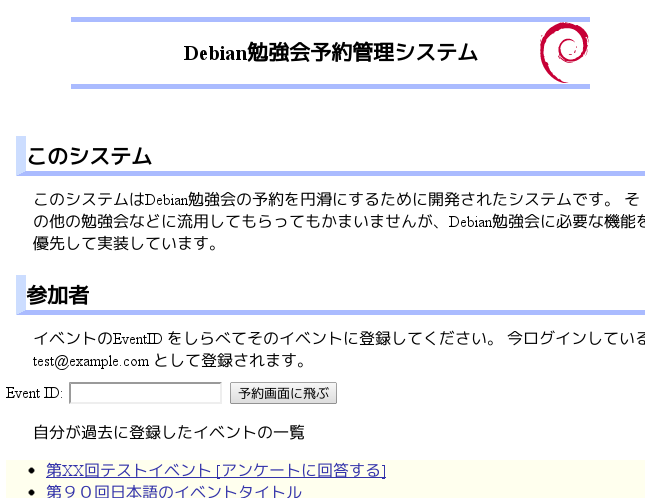
\includegraphics[width=1\hsize]{image201304/enquetereminder.png}
\end{wrapfigure}

$B%"%s%1!<%H$rAwIU$7$F$$$^$9$,!"8=>u%a!<%k$GDLCN$7$F$$$k$N$_$G!"%a!<%k$+$i(B
$B$7$+%"%s%1!<%H2sEz$G$-$^$;$s!#(B
$BJY6/2q$KEPO?$7$F$$$k>l9g$K%"%s%1!<%H$r0MMj$7$F$b%a!<%k$,$H$I$$$F$$$J$$$H(B
$B$+%a!<%k$K5$$E$$$F$$$J$$$H$$$&%U%#!<%I%P%C%/$r$b$i$$$^$7$?!#(B

$B$7$+$7$J$,$i%a!<%kDLCN0J30$GJY6/2q$N$"$H$K%&%'%V%Z!<%8$KMh$F$b$i$&$H$$$&(B
$B$N$OFq$7$$$H;W$&$N$G$9$,!"$b$N$O;n$7$H$$$&;v$G%H%C%W%Z!<%8$K%j%s%/$rI=<((B
$B$9$k$h$&$K$7$F8+$^$7$?!#;22C$7$F$$$k%$%Y%s%H$G%"%s%1!<%H$N<ALd$,:n@.$5$l(B
$B$F$$$F%"%s%1!<%H$N2sEz$,$^$@$J$5$l$F$$$J$$>l9g$K%"%s%1!<%H$N%j%s%/$rI=<((B
$B$7$^$9!#(B


\subsection{$BJY6/2q$KEPO?$7$?;~9o(B}

SVG$B$G$J$K$,$G$-$k$N$+;n$7$F$_$kJY6/$N$D$$$G$KJY6/2q44;vMQ$N%Z!<%8$K%0%i(B
$B%U$r=P$9$h$&$K$7$F8+$^$7$?!#;~9o$r#1#0$KJ,3d$7$F$=$l$>$l$N;~9o$K$*$$$F$N(B
$BEPO?$NIQEY$N?d0\$r$_$l$k$h$&$K$7$F$$$^$9!#$3$N%0%i%U$r8+$k$3$H$G$I$N%$%Y(B
$B%s%H$G$$$D$4$m2??MEPO?$7$?$N$+$,$o$+$j$^$9!#(B
$B;n$7$K:G6a$NFs2s$r8+$F$_$?$N$G$9$,$1$C$3$&0c$$$^$9$M!#(B

HTML5 $B$K$*$$$F(BSVG$B$N2hA|$r$&$a$3$`$N$O7k9=4JC1$G!"$=$N$^$^(BSVG$B%?%0$rKd$a9~$a(B
$B$P$$$$$@$1$G$9!#(Binkscape$B$NEG$/(BSVG$B$r$_$F<j=q$-$OL5M}$+$J$H;W$C$F$$$?$N$G(B
$B$9$,4pK\E*$J5-K!$@$1$G$"$l$P<j=q$-$9$k$N$b0-$/$O$J$$$H;W$($k=q<0$G$7$?!#(B
\index{svg}

\begin{commandline}
 <svg width="800" height="120">
	  <text x="0" y="120">2012-11-03</text>
	  <text x="400" y="120">2012-11-17</text>
	  <text x="0" y="100">0</text>
	  <text x="0" y="16">6</text>
	  <polyline points="
 0,83.3333333333
 50,66.6666666667
 100,83.3333333333
 150,100.0
 200,100.0 
 250,100.0 
 300,100.0 
 350,100.0 
 400,0.0 
 450,33.3333333333 " 
          fill="none" stroke="#333">
	  </polyline>
    </svg>
\end{commandline}

\begin{figure}[ht]
\begin{minipage}{0.5\hsize}
 \begin{center}
  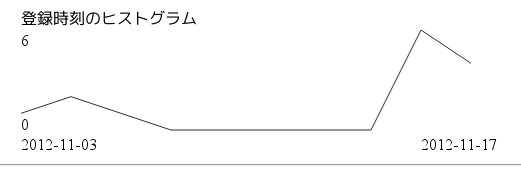
\includegraphics[width=1\hsize]{image201304/attendgraph1.png}
 \end{center} 
 \caption{2012$BG/(B11$B7n$NJY6/2q$NEPO?;~9o(B}
\end{minipage}
\begin{minipage}{0.5\hsize}
\begin{center}
  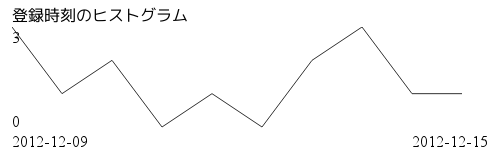
\includegraphics[width=1\hsize]{image201304/attendgraph2.png}
\end{center} 
\caption{2012$BG/(B12$B7n$NJY6/2q$NEPO?;~9o(B}
\end{minipage}
\end{figure}

\subsection{$B%3%_%C%H?t(B}

\begin{wrapfigure}{r}{30zw}
\begin{center}
\includegraphics[width=1\hsize]{image201304/util-gae-commits.eps}
\end{center}
\caption{$B3F;MH>4|Kh$K$*$1$k(Butil/gae$B%G%#%l%/%H%j$N(Bgit$B%3%_%C%H?t(B}
\end{wrapfigure}

$B5$$K$J$C$?$N$G%3%_%C%H?t$N%0%i%U$r:n@.$7$F$_$^$7$?!#;MH>4|$4$H$K%W%m%C%H(B
$B$7$F$$$^$9!#G/Kv$K=8Cf$7$F%3%_%C%H$7$F$$$k$N$,8+$F<h$l$^$9!#$7$P$i$/$$$8$C(B
$B$F$J$$5$$,$7$F$$$^$7$?$,G/$K0l2s$/$i$$$O4hD%$C$F$$$8$C$F$k;~4|$,$"$k$_$?(B
$B$$$G$9$M!#0lG/$r?6$jJV$k$D$$$G$K$$$m$$$mO.$j$?$/$J$k$N$+$b$7$l$^$;$s!#(B


%-------------------------------------------------------------------------------
\dancersection{debootstrap$B$rM-8z3hMQ$7$F$_$h$&(B}{$B?yK\E5=<(B}
%-------------------------------------------------------------------------------
\index{debootstrap}

debian$B$N%$%s%9%H!<%k=hM}$K;H$&(Bdebootstrap$B%3%^%s%I$N1~MQNc$H$7$F3+H/4D6-@0Hw!"%5!<%PMQES!"AH$_9~$_MQES!"0[<o(BOS$BMxMQ$H$^$H$a$F$_$^$7$?!#(B

\subsection{$B2>A[2=5;=Q$K$D$$$F(B}
$B:G6a(BKVM$B$r;vNc$H$9$k!V2>A[2=!W$H$$$&8@MU$r$h$/J9$/$h$&$K$J$j$^$7$?!#2>A[2=$K$b$$$/$D$+$N<oN`$,$"$k$H;W$$D4$Y$F$_$?$H$3$m!"0J2<$NNc$,8+$D$+$j$^$7$?!#:#2s$O!"%3%s%F%J7?2>A[2=$KCeL\$7$F$$$-$^$9!#(B

\begin{table}[hb]
  \begin{tabular}{|l|p{10em}|p{20em}|} \hline
    $B2>A[2=5;=Q(B & $B<BAuNc(B & $B2>A[2=4D6-$NFCD'(B \\ \hline
    $B40A42>A[2=(B($B%(%_%e%l!<%7%g%s7?(B) & QEMU$B!"(BVirtualBox & $B4{B8$N(BOS$B$rL5=$@5$N$^$^%2%9%H4D6-$H$7$FF0:n$5$;$k!#%[%9%H(BOS$B$GF0:n$9$k2>A[2=%"%W%j%1!<%7%g%s$,%(%_%e!<%7%g%s$9$k!#(B \\ \hline
    $B40A42>A[2=(B($B%O%$%Q!<%P%$%67?(B) & KVM & $B4{B8$N(BOS$B$rL5=$@5$N$^$^%2%9%H4D6-$H$7$FF0:n$5$;$k!#(BCPU$BEy$N2>A[2=5!G=$r;H$&$3$H$G%[%9%H4D6-$K$*$1$k%*!<%P!<%X%C%I$r6KNO8:$i$7$F$$$k!#(B \\ \hline
    $B=`2>A[2=(B & Xen & $B%[%9%H4D6-$H$d$j$H$j$9$k(BAPI$B$rMxMQ$G$-$k$h$&$K=$@5$,F~$C$?(BOS$B$r%2%9%H(BOS$B$H$7$FF0:n$5$;$kJ}<0!J!a4{B8$N(BOS$B$=$N$^$^$G$OF0$+$J$$!K(B \\ \hline
    $B%3%s%F%J7?2>A[2=(B & OpenVZ$B!"(BLXC$B!"(BFreeBSD jail & $B%[%9%H4D6-$H%2%9%H4D6-$OF10l%+!<%M%k$GF0:n$7$D$D!"%[%9%H4D6-$+$iJ,N%$7$?%2%9%H4D6-$rDs6!$9$k!#(B  \\ \hline
  \end{tabular}
\end{table}

\subsection{debian$B$K$*$1$k%3%s%F%J4D6-$N:n$jJ}(B}

\subsubsection{debootstrap}
debian$B$K$*$$$F%3%s%F%J7?2>A[2=$N4D6-$r9=C[$9$k5!G=$H$7$F(Bdebootstrap$B$,$"$j$^$9!#(Bdebootstrap$B$r<B9T$9$k$H!"(Bdebian$B$r%$%s%9%H!<%k$7$?$H$-$N%k!<%H%G%#%l%/%H%j9=B$$rG$0U$N%Q%9$K:n@.$9$k$3$H$,$G$-$^$9!#(B

debootstrap$B$N%$%s%9%H!<%k$O0J2<$N(Bapt-get$B%3%^%s%I$G<B9T$G$-$^$9!#(Bdeboostrap$B$K$O(Bdebootstrap$B!J(Bsh$B%9%/%j%W%H$G<BAu!K$H(Bcdebootsrap$B!J(BC$B8@8l$G<BAu!K$N#2<oN`$N%3%^%s%I$,$"$j$^$9!#(B

\begin{commandline}
$ sudo apt-get install debootstrap cdebootstrap
$ sudo mkdir -p /srv/chroot
$ cd /srv/chroot
$ sudo debootstrap --arch=amd64 sid ./mysid http://ftp.jp.debian.org/debian
$ ls mysid
bin   dev  home  lib64  mnt  proc  run   selinux  sys  usr
boot  etc  lib   media  opt  root  sbin  srv      tmp  var
\end{commandline}

\subsubsection{chroot$B%3%^%s%I(B}
debootstrap$B$G:n@.$7$?%3%s%F%J4D6-$G%W%m%0%i%`$r<B9T$7$?$$$N$G$9$,!"4D6-JQ?t$H%G%#%l%/%H%j$NG[CV$,9g$o$J$$$?$a$&$^$/%3%^%s%I$r<B9T$9$k$3$H$,$G$-$^$;$s!#$=$3$G(Bchroot$B%3%^%s%I$r;H$$$^$9!#(B\footnote{chroot$B%7%9%F%`%3!<%k$O(B1982$BG/$K%S%k!&%8%g%$$,:n@.$7$?$b$N$,5/8;$H$5$l$F$$$^$9!#%S%k!&%8%g%$$O%W%m%0%i%`$r%/%j!<%s%S%k%I$G$-$k4D6-$,$[$7$+$C$?$?$aDL>oMxMQ$N4D6-$HJ,N%$9$k<jCJ$H$7$F3+H/$7$?$H8@$o$l$F$$$^$9!#(B} \footnote{$B%/%j!<%s%S%k%IL\E*$G(Bchroot$B%3%^%s%I$r;H$&<jK!$G$O(Bdebian$B%Q%C%1!<%8$N%S%k%I$K$b;H$o$l$F$$$^$9!#(B}

chroot$B%3%^%s%I$r<B9T$9$k$H%k!<%H%G%#%l%/%H%j$G$J$$>l=j$r$"$?$+$b%k!<%H%G%#%l%/%H%j$G$"$k$h$&$K8+$;$k$3$H$,$G$-$^$9!#$3$l$K$h$jIaDL$K(Bdebian$B$r%$%s%9%H!<%k$7$?>uBV$N%W%m%0%i%`$NG[CV$H(BPATH$B4D6-JQ?t$,$&$^$/9g$$!"%3%s%F%J4D6-$N%W%m%0%i%`$r<B9T$G$-$k$h$&$K$J$j$^$9!#(B

\begin{commandline}
$ sudo chroot /srv/chroot/mysid
# pwd
/
# ls
bin   dev  home  lib64  mnt  proc  run   selinux  sys  usr
boot  etc  lib   media  opt  root  sbin  srv      tmp  var
\end{commandline}

chroot$B%3%^%s%I$K$b8=:_$G$O$$$/$D$+$NGI@8HG$,$"$j$^$9!#(B

\begin{itemize}
  \item chroot
  \begin{itemize}
    \item $B85AD(Bchroot$B!#<B9T$9$k$K$O(Broot$B8"8B$,I,MW!#(B
  \end{itemize}
  \item dchroot
  \begin{itemize}
    \item chroot$B$r0lHL%f!<%6$G<B9T$G$-$k$h$&$K2~NI$7$?HG!#(B($B$H$O$$$((Bdebootstrap$B$H@_Dj%U%!%$%k:n@.$O(Broot$B8"8B$,I,MW(B)
  \end{itemize}
  \item schroot
  \begin{itemize}
    \item dchroot$B$N%;%-%e%j%F%#%l%Y%k$r8~>e$5$;$?2~NIHG!#(B
  \end{itemize}
\end{itemize}

$B:#EY$O(Bschroot$B%3%^%s%I$G%3%s%F%J4D6-$KF~$C$F$_$^$9!#(B

\begin{commandline}
$ sudo apt-get install schroot
$ cd /etc/schroot
$ sudo vi schroot.conf

[mysid]
description=my sid for devel
type=directory
directory=/srv/chroot/mysid
users=norimitu
root-groups=root
personality=linux
preserve-environment=true

$ schroot -c mysid
W: Failed to change to directory $B!F(B/etc/schroot$B!G(B: No such file or directory
I: The directory does not exist inside the chroot.  Use the --directory option to run the command in a different directory.
W: Falling back to directory $B!F(B/home/norimitu
$ ls -la /srv
total 8
drwxr-xr-x  2 root root 4096 Apr 14 02:59 .
drwxr-xr-x 22 root root 4096 Apr 14 03:04 ..

$B!J2?$b$J$$$G$9!#(Bchroot$B4D6-$KF~$C$F$$$^$9!K(B
$ cd /home/norimitu
$ ls
(chroot$B85$N%[%9%H4D6-$N%U%!%$%k$,=P$F$/$k!#(B)
\end{commandline}

$BD>46E*$K$O(Bchroot$B%3%^%s%I$NJ}$,$o$+$j$d$9$$$G$9!#(B

schroot$B%3%^%s%I$N>l9g$O!"(Bschroot$B$7$?4D6-Fb$N%[!<%`%G%#%l%/%H%j$O%[%9%H4D6-$N%[!<%`%G%#%l%/%H%j$H(Bbind$B$5$l$^$9!#$=$N$?$a!"%[%9%H4D6-$K$"$k%U%!%$%k$r(Bschroot$B$7$?4D6-$+$i$=$N$^$^FI$_=q$-$G$-$^$9!#!J(Bchroot$B$N>l9g$O$=$&$$$&;EAH$_$,$J$$$?$a!"%3%T!<$9$kI,MW$,$"$k!#!K(B

\subsection{debootstrap$B$N;H$$$I$3$m(B}

debootstrap$B$r;H$&$H2?$,JXMx$J$N$+;H$$$I$3$m$NNc$r>e$2$F$_$^$9!#(B

\subsubsection{$B@83h4D6-$H3+H/(B($B%F%9%H(B)$B4D6-$rJ,N%$9$k(B}

$BIaCJ;HMQ$9$k4D6-$O(Bstable$B$rMxMQ$9$k$,!"%P!<%8%g%sEy$NET9g$GItJ,E*$K(Bsid$B$GDs6!$5$l$F$$$k%Q%C%1!<%8$rMxMQ$7$?$$>l9g$,$"$j$^$9!#$=$N>l9g!"A0=R$7$?J}K!$G%3%s%F%J4D6-$r:n@.$7!"(Bchroot$B$9$l$PMxMQ$G$-$^$9!#(B

\subsubsection{$B%3%s%F%JFb$G0[$J$k(BCPU$B%"!<%-%F%/%A%c$N4D6-$rF0$+$9(B}

debootstrap$B$7$?%3%s%F%J4D6-$ODL>o%[%9%H4D6-$GF0:n$9$k(BCPU$B%"!<%-%F%/%A%c$G9=C[$7$^$9!#(Bchroot$B%3%^%s%I$G%3%s%F%J4D6-$KF~$C$F$$$k>l9g$G$b%+!<%M%k$O%[%9%H(BOS$B$HF1$8$?$a!"0[$J$k(BCPU$B%"!<%-%F%/%A%c$N%P%$%J%j$r%M%$%F%#%V$K<B9T$G$-$J$$$?$a$G$9!#(B

amd64$B%+!<%M%k$r<B9T$7$F$$$k%^%7%s$N>l9g!"(Bi386$B%P%$%J%j$O<B9T$G$-$^$9$N$G(Bi386$B4D6-$N%3%s%F%J4D6-$r9=C[$9$l$P<B9T$G$-$^$9!#(B

$B;d$O=tHL$NET9g$G(Bi386$B$N(Bpostgresql-9.1$B$rF0$+$7$F(BVPS$B$X%l%W%j%1!<%7%g%s$7$F$$$^$9$,!"(Bamd64$B$H(Bi386$B4V$H$$$C$?(BCPU$B%"!<%-%F%/%A%c$,0[$J$k>l9g$K%l%W%j%1!<%7%g%s$,$G$-$J$$;EMM$H$J$C$F$$$k$?$a!"(BVPS$B$N%[%9%H(BOS$B$O(Bamd64$B!"%3%s%F%JFb$G(Bi386$B4D6-$rF0$+$7$F%l%W%j%1!<%7%g%s$7$F$$$^$9!#(B

% personality flags $B$b9M$($k$HB?J,(B linux32 $B%3%^%s%I;H$C$?$[$&$,NI$$$H;W(B
% $B$&(B --dancerj
\begin{commandline}
$ sudo mkdir -p /srv/chroot
$ cd /srv/chroot
$ sudo debootstrap --arch=i386 sid ./mysid-i386 http://ftp.jp.debian.org/debian
$ sudo chroot ./mysid-i386
# uname -a
Linux www6368uj 3.2.0-4-amd64 #1 SMP Debian 3.2.41-2 x86_64 GNU/Linux
# apt-get install file
# file /bin/ls
/bin/ls: ELF 32-bit LSB executable, Intel 80386, version 1 (SYSV),
dynamically linked (uses shared libs), for GNU/Linux 2.6.26,
BuildID[sha1]=0x498625fc854816515ec12819544ebedff51d5c32, stripped
\end{commandline}

$B!!$^$?!"(Bchroot$B$H(BQEMU$B$rAH$_9g$o$;$k$3$H$K$h$j!"%[%9%H(BOS$B$N%+!<%M%k$G$OF0:n$7$J$$(BCPU$B%"!<%-%F%/%A%c$N%3%s%F%J4D6-$r(BQEMU$B$r;H$C$?%(%_%e%l!<%H$GF0:n$5$;$k$3$H$,$G$-$^$9!#:G6aN.9T$j$N0B2A$J(BARM$B%\!<%I$G(Bdebian$B$rF0:n$5$;$k$?$a$N%G%#%l%/%H%j%D%j!<$r:n@.$9$k$N$KJXMx$G$9!#(B\footnote{$B<B:]$K(BARM$B%\!<%I>e$G(Bdebian$B$r5/F0$5$;$k$?$a$K$O(BSD$B%+!<%IEy$X$N%U%!%$%k%7%9%F%`:n@.!"%+!<%M%k$d%I%i%$%P$N:n@.!"%V!<%H%m!<%@!<$N=q$-9~$_Ey!"?'!9$d$i$J$$$HF0$-$^$;$s!#(B}

$B!!%[%9%H4D6-$H0[$J$k(BCPU$B%"!<%-%F%/%A%c$N%3%s%F%J4D6-$r(Bchroot$B$9$k>l9g!"0J2<$N<j=g$G<B9T$9$kI,MW$,$"$j$^$9!#(B

\begin{itemize}
  \item debootstrap$B$O!V(B--foreign$B!W0z?t$rEO$7$F<B9T$9$k$3$H(B
  \item $B%3%s%F%J4D6-Fb$K!V(Bqemu-*-static$B!W%U%!%$%k$r%3%T!<$7$F$*$/$3$H!JNc!'(Bqemu-arm-static$B!K(B
  \item chroot$B$GF~$C$?8e$G(Bdebootstrap$B$N(Bsecond stage$B$r<B9T$9$k$3$H(B
\end{itemize}

\begin{commandline}
$ sudo apt-get install binfmt-support qemu qemu-user-static debootstrap
$ sudo mkdir -p /srv/chroot
$ cd /srv/chroot
$ sudo debootstrap --foreign --arch=armel wheezy ./armdev1 http://ftp.jp.debian.org/debian
$ sudo chroot ./armdev1
chroot: $B%3%^%s%I(B `/bin/bash' $B$N<B9T$K<:GT$7$^$7$?(B: No such file or directory

$ sudo cp /usr/bin/qemu-arm-static /srv/chroot/armdev1/usr/bin/
$ sudo chroot armdev1
I have no name!@hostname:/#
Linux hostname 3.2.0-4-amd64 #1 SMP Debian 3.2.41-2 armv7l GNU/Linux

I have no name!@hostname:/# apt-get update
bash: apt-get: command not found
I have no name!@hostname:/# ls /debootstrap
arch  debootstrap      debpaths        functions  suite
base  debootstrap.log  devices.tar.gz  required   suite-script
I have no name!@hostname:/# /debootstrap/debootstrap --second-stage
I: Installing core packages...
I have no name!@hostname:/# apt-get update
Reading package lists...

I have no name!@hostname:/# vi /etc/apt/sources.list

deb http://ftp.jp.debian.org/debian wheezy main
deb-src http://ftp.jp.debian.org/debian wheezy main

deb http://security.debian.org/ wheezy/updates main
deb-src http://security.debian.org/ wheezy/updates main

I have no name!@hostname:/# apt-get update
I have no name!@hostname:/# apt-get install file
I have no name!@hostname:/# file /bin/ls
/bin/ls: ELF 32-bit LSB executable, ARM, version 1 (SYSV),
dynamically linked (uses shared libs), for GNU/Linux 2.6.26,
BuildID[sha1]=0x5bc97dbca9ac168932d898a5e2eaf68e8fde5e16, stripped
\end{commandline}


\subsubsection{$B%5!<%P$G$?$/$5$s$N%3%s%F%J$r>oCs$5$;$FF0$+$7$?$$(B}

$B:#$^$G$N%3%s%F%J4D6-$O<j$G%3%^%s%I$r<B9T$9$k$3$H$G%3%s%F%J4D6-$KF~$C$F$$$^$7$?!#%3%s%F%J4D6-$r%5!<%P$N$h$&$KF0$+$7$?$$$H$$$&%K!<%:$b$"$j$^$9!#:#2s$O(BDebian GNU/Linux wheezy amd64$B>e$G(BLXC$B!J(BLinux Containers$B!K$rMQ$$$F%3%s%F%J4D6-$r>oCs$5$;$F$_$^$9!#(B

$B$^$:%[%9%H4D6-$N@_Dj$H4D6-$r3NG'$7$^$9!#(B

\begin{commandline}
$ sudo apt-get install lxc
$ sudo vi /etc/fstab

$B!JDI5-$7$^$9!K(B
cgroup  /sys/fs/cgroup  cgroup  defaults  0   0

$ sudo mount -a
$ lxc-checkconfig
Kernel config /proc/config.gz not found, looking in other places...
Found kernel config file /boot/config-3.2.0-4-amd64
--- Namespaces ---
Namespaces: enabled
Utsname namespace: enabled
Ipc namespace: enabled
Pid namespace: enabled
User namespace: enabled
Network namespace: enabled
Multiple /dev/pts instances: enabled

--- Control groups ---
Cgroup: enabled
Cgroup clone_children flag: enabled
Cgroup device: enabled
Cgroup sched: enabled
Cgroup cpu account: enabled
Cgroup memory controller: enabled
Cgroup cpuset: enabled

--- Misc ---
Veth pair device: enabled
Macvlan: enabled
Vlan: enabled
File capabilities: enabled

Note : Before booting a new kernel, you can check its configuration
usage : CONFIG=/path/to/config /usr/bin/lxc-checkconfig
\end{commandline}

LXC$B$GF0:n$9$k%3%s%F%J4D6-$N%M%C%H%o!<%/$O%[%9%H4D6-$H%V%j%C%8@\B3$9$kI,MW$,$"$j$^$9!#(B

$B$3$3$G$O(Beth0$B$O$=$N$^$^$G%V%j%C%8%G%P%$%9$r#1$D:n@.$7!"(BLXC$B$N%3%s%F%J4D6-$O%V%j%C%8%G%P%$%9$N(BNAT$B4D6-2<$GF0:n$9$k$3$H$H$7$^$9!#(B\footnote{http://wiki.debian.org/LXC/SimpleBridge}

\begin{commandline}
$ sudo vi /etc/sysctl.conf

$B!JJQ99!K(B
net.ipv4.ip_forward=1

$ sudo sysctl -p
net.ipv4.ip_forward = 1

$ vi br-lxc.sh
# script to setup a natted network for lxc guests
CMD_BRCTL=/sbin/brctl
CMD_IFCONFIG=/sbin/ifconfig
CMD_IPTABLES=/sbin/iptables
CMD_ROUTE=/sbin/route
NETWORK_BRIDGE_DEVICE_NAT=lxc-bridge-nat
HOST_NETDEVICE=eth0
PRIVATE_GW_NAT=192.168.20.1
PRIVATE_NETMASK=255.255.255.0
PRIVATE_NETWORK=192.168.20.0/24

${CMD_BRCTL} addbr ${NETWORK_BRIDGE_DEVICE_NAT}
${CMD_BRCTL} setfd ${NETWORK_BRIDGE_DEVICE_NAT} 0

${CMD_IFCONFIG} ${NETWORK_BRIDGE_DEVICE_NAT} ${PRIVATE_GW_NAT} netmask ${PRIVATE_NETMASK} promisc up

${CMD_IPTABLES} -t nat -A POSTROUTING -o ${HOST_NETDEVICE}  -j MASQUERADE
${CMD_IPTABLES} -A FORWARD -i ${NETWORK_BRIDGE_DEVICE_NAT} -o ${HOST_NETDEVICE} -s ${PRIVATE_NETWORK} -j ACCEPT

$ sudo ./br-lxc.sh
$ sudo ifconfig lxc-bridge-nat
lxc-bridge-nat Link encap:$B%$!<%5%M%C%H(B  $B%O!<%I%&%'%"%"%I%l%9(B fe:24:c3:eb:6d:c3
          inet$B%"%I%l%9(B:192.168.20.1 $B%V%m!<%I%-%c%9%H(B:192.168.20.255  $B%^%9%/(B:255.255.255.0
          inet6$B%"%I%l%9(B: fe80::409a:3cff:fee6:33b0/64 $BHO0O(B:$B%j%s%/(B
          UP BROADCAST RUNNING PROMISC MULTICAST  MTU:1500  $B%a%H%j%C%/(B:1
          RX$B%Q%1%C%H(B:6556 $B%(%i!<(B:0 $BB;<:(B:0 $B%*!<%P%i%s(B:0 $B%U%l!<%`(B:0
          TX$B%Q%1%C%H(B:1121 $B%(%i!<(B:0 $BB;<:(B:0 $B%*!<%P%i%s(B:0 $B%-%c%j%"(B:0
      $B>WFM(B(Collisions):0 TX$B%-%e!<D9(B:0
          RX$B%P%$%H(B:543131 (530.4 KiB)  TX$B%P%$%H(B:95778 (93.5 KiB)
\end{commandline}

$B%3%s%F%J$r:n@.$7$^$9!#(BLXC$B$K$*$1$k%3%s%F%J$O(B ``\texttt{/var/lib/lxc}''$B%G%#%l%/%H%j$N2<$K$G$-$^$9!#(B

\begin{commandline}
$ sudo lxc-create -n lxc-deb1 -t debian
$B!!!J%@%$%"%m%07A<0$G%$%s%9%H!<%k$9$k%P!<%8%g%s$d%@%&%s%m!<%I@h%_%i!<$N(BURL$B!"(B
$B!!!!(Broot$B%Q%9%o!<%I$,J9$+$l$k$N$GEz$($k!K(B 

$ cd /var/lib/lxc/lxc-deb1
$ ls
config    rootfs
$ sudo vi config

$B!JDI5-$7$^$9!K(B
## Network
lxc.utsname = lxc-deb1
lxc.network.type = veth
lxc.network.flags = up

# that's the interface defined above in host's interfaces file
lxc.network.link = lxc-bridge-nat

# name of network device inside the container,
# defaults to eth0, you could choose a name freely
# lxc.network.name = lxcnet0

lxc.network.hwaddr = 00:FF:AA:00:00:01

# the ip may be set to 0.0.0.0/24 or skip this line
# if you like to use a dhcp client inside the container
lxc.network.ipv4 = 192.168.20.101/24
\end{commandline}

LXC$B%3%s%F%JFb$G(Bsshd$B$,5/F0$9$k$h$&@_Dj$7$F$*$-$^$9!#(B

\begin{commandline}
$ sudo cp /etc/resolv.conf /var/lib/lxc/lxc-deb1/rootfs/etc/
$ sudo vi /var/lib/lxc/lxc-deb1/rootfs/etc/ssh/sshd_config

$B!JJQ99A0!K(B  #ListenAddress 0.0.0.0
$B!JJQ998e!K(B  ListenAddress 192.168.20.101 
\end{commandline}

LXC$B%3%s%F%J$r5/F0$7$^$9!#(B``-d''$B%*%W%7%g%s$O%P%C%/%0%i%&%s%I$G5/F0$5$;$k%*%W%7%g%s$G$9!#$3$l$G%3%s%F%J4D6-$,>oCs$7$FF0:n$9$k$h$&$K$J$j$^$9!#(B

\begin{commandline}
$ sudo lxc-start -n lxc-deb1
Using makefile-style concurrent boot in runlevel 2.
Starting OpenBSD Secure Shell server: sshdCould not load host key: /etc/ssh/ssh_host_rsa_key
Could not load host key: /etc/ssh/ssh_host_dsa_key

$B$J$<$+(Bssh$B80$r:n$k=hM}$,<+F0<B9T$5$l$:;_$^$C$F$7$^$&$?$a!"<jF0$G:n$C$F$_$k!#(B
$ sudo chroot /var/lib/lxc/lxc-deb1/rootfs ssh-keygen -t dsa -f /etc/ssh/ssh_host_dsa_key
$ sudo chroot /var/lib/lxc/lxc-deb1/rootfs ssh-keygen -t rsa -f /etc/ssh/ssh_host_rsa_key

$ sudo lxc-start -n lxc-deb1 -d
$ ssh root@192.168.20.101
root@lxc-deb1:~#

$B!!%m%0%$%s$G$-$^$7$?!#(B

$ sudo lxc-stop -n lxc-deb1
\end{commandline}

\subsubsection{$B0[$J$k(BOS$B>e$G(Bdebian$B$r9=C[$9$k(B}

debootstrap$B$O0[$J$k(BOS$B>e$G(Bdebian$B$r9=C[$9$k$3$H$,$G$-$^$9!#$3$3$G$O!"(BFreeBSD-8.3-RELEASE amd64$B$N(Bjail$B5!G=$rMQ$$$F(Bkfreebsd-amd64$B$r(Bprisoner$B$H$7$FF0$+$7$F$_$^$9!#(B\footnote{http://blog.vx.sk/archives/22-Updated-Tutorial-Debian-GNUkFreeBSD-in-a-FreeBSD-jail.html}

$B$^$:$O(Bjail$B4D6-$r:n@.$9$k$?$a$N%D!<%k$r%$%s%9%H!<%k$7$^$9!#(B

OS$B$,0[$J$k$H(Bdebootstrap$B%3%^%s%I$,$J$$$?$a!"(Btarball$B!JCf?H$O(Bsh$B%9%/%j%W%HHG!K$r%@%&%s%m!<%I$7$F<B9T$7$^$9!#(B\footnote{ports$B$G(B/usr/ports/sysutils/debootstrap$B$b$"$j$^$9$N$G$=$A$i$r;H$C$F$b$$$$$G$9(B}

\begin{commandline}
> cd
> wget http://ftp.jp.debian.org/debian/pool/main/d/debootstrap/debootstrap_1.0.48.tar.gz
> tar xf debootstrap_1.0.48.tar.gz
> cd debootstrap-1.0.48
# su
# setenv DEBOOTSTRAP_DIR `pwd`
# ./debootstrap --arch=kfreebsd-amd64 wheezy /usr/jails/jailkfdeb http://ftp.jp.debian.org/debian
# kldload fdescfs linprocfs linsysfs tmpfs
# umount /usr/jails/jailkfdeb/dev/fd
# umount /usr/jails/jailkfdeb/dev
# mount -t linprocfs linprocfs /usr/jails/jailkfdeb/proc
# mount -t linsysfs linsysfs /usr/jails/jailkfdeb/sys
# mkdir -p /usr/jails/jailkfdeb/lib/init/rw
# mount -t tmpfs tmpfs /usr/jails/jailkfdeb/lib/init/rw
# cp /etc/resolv.conf /usr/jails/jailkfdeb/etc/resolv.conf
\end{commandline}

\begin{commandline}
> sudo portsnap fetch
> sudo portsnap update
> cd /usr/ports/sysutils/ezjail
> sudo make
> sudo make install

> sudo touch /etc/fstab.jailkfdeb
  $B!J$3$N%U%!%$%k$,$J$$$H%(%i!<$K$J$k$?$a$H$j$"$($::n@.$7$^$9!K(B
> vi /etc/rc.conf
$B!JDI5-$7$^$9!K(B
ifconfig_em0_alias0="inet 192.168.1.63/32"

> ifconfig em0 192.168.1.63 netmask 255.255.255.255 alias
> vi /usr/local/etc/ezjail/jailkfdeb

# To specify the start up order of your ezjails, use these lines to
# create a Jail dependency tree. See rcorder(8) for more details.
#
# PROVIDE: standard_ezjail
# REQUIRE:
# BEFORE:
#

export jail_jailkfdeb_hostname="jailkfdeb"
export jail_jailkfdeb_ip="192.168.1.63"
export jail_jailkfdeb_rootdir="/usr/jails/jailkfdeb"
export jail_jailkfdeb_exec_start="/etc/init.d/rc 3"
export jail_jailkfdeb_exec_stop=""
export jail_jailkfdeb_flags="-l -u root"
export jail_jailkfdeb_mount_enable="YES"
export jail_jailkfdeb_devfs_enable="YES"
export jail_jailkfdeb_devfs_ruleset="devfsrules_jail"
export jail_jailkfdeb_procfs_enable="YES"
export jail_jailkfdeb_fdescfs_enable="YES"


> sudo /usr/local/etc/rc.d/ezjail start jailkfdeb
Configuring jails:.
Starting jails: jailkfdeb.
> jls
   JID  IP Address      Hostname                      Path
    11  192.168.1.63    jailkfdeb                     /usr/jails/jailkfdeb
> jexec 11 /bin/sh

$B!J$3$3$+$i%3%s%F%J4D6-$NCf$G$9!K(B

# uname -irps
GNU/kFreeBSD 8.3-RELEASE-p6 amd64 Intel(R) Core(TM) i5-2500S CPU @ 2.70GHz
# vi /etc/apt/sources.list

deb http://ftp.jp.debian.org/debian wheezy main contrib non-free
deb-src http://ftp.jp.debian.org/debian wheezy main contrib non-free

# apt-get update
# apt-get install openssh-server
# vi /etc/ssh/sshd_config

$B=$@5A0!K(B  #ListenAddress 0.0.0.0
$B=$@58e!K(B  ListenAddress 192.168.1.63

# /etc/init.d/ssh restart
# passwd
# exit

$B!J%3%s%F%J4D6-$+$i%[%9%H4D6-$KLa$j$^$9!K(B

> ssh root@192.168.1.63 
\end{commandline}

ssh$B$G%3%s%F%J4D6-$K%m%0%$%s$G$-$^$7$?!#(B

\subsection{$B;29M>pJs(B}

\begin{itemize}
  \item{Debian Wiki Schroot http://wiki.debian.org/Schroot}
  \item{Debian Wiki LXC http://wiki.debian.org/LXC}
  \item{Debian Wiki EmDebianCrossDebootstrap http://wiki.debian.org/EmDebian/CrossDebootstrap}
  \item{$B4X@>%(%j%"(BDebian$BJY6/2q(B 2009$BG/(B04$B7n9f!V(BDebian $B$r?75,$K(B install $B$7$F$+$i>oMQ4D6-$K$9$k$^$G!W(B $B:4!9LZMNJ?(B}
  \item{Updated Tutorial: Debian GNU/kFreeBSD in a FreeBSD jail  http://blog.vx.sk/archives/22-Updated-Tutorial-Debian-GNUkFreeBSD-in-a-FreeBSD-jail.html}
\end{itemize}

\dancersection{Samba $B$G(B Linux $B$NG'>Z$r(B Windows $B$KE}9g$7$F$_$?$j(B}{$B$?$+$O$7$b$H$N$V(B}
\index{samba}

\subsection{$BL5;|Ha$J0l8@!"8@$o$l$^$;$s$+(Bw}
Windows$B$NBg72$NCf$G(BLinux$B%5!<%P$r1?MQ$7$F$$$k$H$h$/8@$o$l$k$N$,!"!V$=$N(B(Linux)$B%5!<%P$NG'>Z!"(BActive Directory$B$G$G$-$J$$$N(B?$B!W$H$$$&BgJQL5;|Ha$J(B($B>P(B)$B0l8@$G$O$J$$$G$7$g$&$+!#$H$$$&$3$H$G!":#2s$O(BSamba$B$r;H$C$F(BLinux$B%5!<%P$NG'>Z$r(BWindows$B$KE}9g$9$kJ}K!$K$D$$$F!"$$$m$$$m$4>R2p$7$F$$$-$?$$$H;W$$$^$9!#(B
\index{active directory}

\subsection{Samba$B$C$F(B$\cdots \cdots$}
$B0l1~@bL@$7$F$*$-$^$9$H!"(BDebian$B$r4^$`(BUNIX$B7O(B OS $B>e$G%U%!%$%k6&M-$r$O$8$a$H$9$k(BWindows$B%5!<%P$N3F<o5!G=$r<B8=$9$k%*!<%W%s%=!<%9$N%=%U%H%&%'%"$G$9!#85!9$O%U%!%$%k6&M-!"%W%j%s%?6&M-$N5!G=$+$i=PH/$7$F$$$^$9$,!":G6a$G$O(BWindows$B$NCf3K5!G=$G$"$k(BActive Directory$B$N%I%a%$%s%3%s%H%m!<%i5!G=$d!"(BWindows$B%I%a%$%s$N%/%i%$%"%s%H5!G=$J$I!"B?$/$N5!G=$r<BAu$7$F$$$^$9!#(B

$B$?$@!"$=$N$"$?$j$N5!G=$N>R2p$r$7$F$$$k$H!"(BSamba$B$H$$$&$h$j(BWindows$B$N5!G=$N>R2p$K$J$C$F$7$^$&$N$G!":#2s$O(BLinux$B%a%$%s$JJ}$G$b<{MW$,$"$j$=$&$J5!G=$H$$$&$3$H$G!"G'>ZE}9g$r<h$j>e$2$F$_$^$7$?!#(B
\index{$B$K$s$7$g$&$H$&$4$&(B@$BG'>ZE}9g(B}

\subsection{Samba $B$G%U%!%$%k%5!<%P$r9=C[$7$F$_$k(B}

$B$^$:$O!"(BSamba$B$N5!G=>R2p$b7s$M$F(BSamba$B$G%U%!%$%k%5!<%P$r9=C[$7$F$_$^$7$g$&!#$3$l$O%Q%C%1!<%8$rE,@Z$K%$%s%9%H!<%k$9$l$P4JC1$G$9!#(B

\begin{commandline}
# apt-get install samba
\end{commandline}

$B%$%s%9%H!<%k$NESCf$GJ9$+$l$k<ALd$O!"(BOK$B$r2!$7$F?J$a$F$*$-$^$7$g$&(B ($B8e$G=$@5$7$^$9(B)$B!#(B

$B%$%s%9%H!<%k$,=*$o$C$?$i!"(B{\tt{/etc/samba/smb.conf}}$B$rJT=8$7$^$9!#%G%U%)%k%H$G$O3F%f!<%6$N%[!<%`%G%#%l%/%H%j$rFI$_<h$j@lMQ$G6&M-$9$k@_Dj$K$J$C$F$$$^$9$N$G!"$3$3$G$OFI$_=q$-2DG=$K$7$F$_$^$9!#(B

\begin{commandline}
[homes]
   comment = Home Directories
   browseable = no

# By default, the home directories are exported read-only. Change the
# next parameter to 'no' if you want to be able to write to them.
   read only = no $B"+(B yes$B$+$iJQ99(B
\end{commandline}

$B$b$&0l$D!"(BSamba$B$G%U%!%$%k6&M-$r9T$&Nc$H$7$F(B{\tt{/tmp}}$B$rFI$_=q$-2DG=$G6&M-$7$F$_$^$7$g$&!#<!$N$h$&$J5-=R$r(B{\tt{smb.conf}}$B$NKvHx$KDI2C$7$^$9!#(B

\begin{commandline}
[tmp-share]
  path = /tmp
  read only = no
\end{commandline}

1$B9TL\$,6&M-L>$N;XDj$G!"$3$3$G$O(B{\tt{tmp-share}}$B$H$$$&L>A0$r;XDj$7$F$$$^$9!#(B2$B9TL\$O6&M-$9$k%Q%9$N;XDj$G!"$3$3$G$O(B{\tt{/tmp}}$B$r;XDj$7$^$7$?!#(B3$B9TL\$OFI$_=q$-2DG=$H$9$k@_Dj$G$9!#%G%U%)%k%H$G$OFI$_<h$j@lMQ$G6&M-$5$l$^$9!#(B

$B<!$K!"$3$N%5!<%P$X$N%"%/%;%9$r9T$&%f!<%6$r:n@.$7$^$9!#(B{\tt{/etc/passwd}}$B$N%f!<%6$K2C$($F!"(BSamba$B$G$O(BWindows$BFH<+$N7A<0$G%O%C%7%e2=$5$l$?G'>Z>pJs$r07$&I,MW$,$"$k$?$a!"(B{\tt{smbpasswd}}$B%3%^%s%I$J$I$rMQ$$!"(B Samba$B%f!<%6$H$$$&FH<+$N%f!<%6$r:n@.$7$F%Q%9%o!<%I$r@_Dj$9$kI,MW$,$"$j$^$9!#(B

\begin{commandline}
# useradd -m local1
# smbpasswd -a local1
New SMB password:
Retype new SMB password:
Added user local1.
\end{commandline}

$B$3$3$G<!$N$h$&$K$7$F(B Samba$B%5!<%P$r:F5/F0$7$F(B{\tt{smb.conf}}$B$N@_DjJQ99$rH?1G$5$;$^$9!#(B

\begin{commandline}
# /etc/init.d/samba restart
Stopping Samba daemons: nmbd smbd.
Starting Samba daemons: nmbd smbd.
\end{commandline}

$B:F5/F08e!"(B{\yen}{\yen}{\sf{Samba}}{\gt{$B%5!<%P$N(B}}{\sf{IP}}{\gt{$B%"%I%l%9(B}} $B$H$7$F(B Windows$B$+$i%"%/%;%9$7$F$_$^$7$g$&!#%U%!%$%"%&%)!<%k$J$I$N@_Dj$r9T$C$F$$$J$1$l$P!"?^(B\ref{fig:monyo-samba03.png}$B$N$h$&$K%f!<%6L>$H%Q%9%o!<%I$rJ9$+$l$k%@%$%"%m%0$,I=<($5$l$^$9!#(B

% --- samba03.png ---%
\begin{figure}[h]
\begin{center}
 \includegraphics[width=.5\hsize]{image201304/samba/monyo-samba03.eps}
 \caption{$B%f!<%6!<L>$H%Q%9%o!<%I$NF~NO%@%$%"%m%0(B}
 \label{fig:monyo-samba03.png}
\end{center}
\end{figure}

$B@h$[$I@_Dj$7$?(Buser1$B$H$$$&%f!<%6L>$H%Q%9%o!<%I$rF~NO$9$l$P!"(Buser1$B$H$$$&%[!<%`%G%#%l%/%H%j$N6&M-$H(B{\tt{tmp-share}}$B$H$$$&@h$[$I:n@.$7$?6&M-$,8+$($F$$$k$O$:$G$9(B($B?^(B\ref{fig:monyo-samba04.png})$B!#(B

% --- samba04.png ---%
\begin{figure}[h]
\begin{center}
 \includegraphics[width=0.8\hsize]{image201304/samba/monyo-samba04.eps}
 \caption{$B%(%/%9%W%m!<%i!<$+$i(BSamba$B%5!<%P$N6&M-$r;2>H(B}
 \label{fig:monyo-samba04.png}
\end{center}
\end{figure}

\subsection{Samba$B$r(BActive Directory(Windows$B%I%a%$%s(B)$B$K;22C$5$;$F$_$k(B}

$B<!$K!"(BSamba$B$r(BActive Directory$B$K;22C$5$;$F!"@h$[$I9=C[$7$?%U%!%$%k%5!<%P$X$N%"%/%;%9$N:]$NG'>Z$r(BWindows$B%I%a%$%s$KE}9g$7$F$_$^$7$g$&!#$3$l$b%Q%C%1!<%8$rE,@Z$K%$%s%9%H!<%k$7$F$$$l$P4JC1$G$9!#(B

$B$^$:<!$N$h$&$K$7$F(B{\tt{/etc/resolv.conf}}$B$rJT=8$7$F!"(BDNS$B%I%a%$%s!"(BDNS$B%5!<%P$H$7$F(BActive Directory$B$N(BDNS $B%5!<%P$r;XDj$7$^$9(B($B$^$@;XDj$7$F$$$J$$>l9g(B) $B!#$3$3$G$O(BW2K8R2AD3.LOCAL$B$H$$$&%I%a%$%sL>$G(BDNS$B%5!<%P$N(BIP$B%"%I%l%9$,(B192.168.135.100$B$G$"$k>l9g$NNc$r<($7$^$9(B(DHCP$B$+$i(BIP$B%"%I%l%9$r<hF@$9$k@_Dj$N>l9g!"$3$N%U%!%$%k$O>e=q$-$5$l$F$7$^$&$N$G!"8GDj(BIP$B$N@_Dj$K$7$F$*$/I,MW$,$"$j$^$9(B):

\begin{commandline}
domain w2k8r2ad3.local $B"+(B Active Directory $B$N%I%a%$%sL>$r;XDj(B
search w2k8r2ad3.local
nameserver 192.168.1.100 $B"+(B Active Directory $B$N(B DNS $B%5!<%P(B ($BDL>o$O%I%a%$%s%3%s%H%m!<%i(B) $B$N(B IP $B%"%I%l%9$r;XDj(B
\end{commandline}

$B$D$$$G!"(B{\tt{smb.conf}}$B%U%!%$%k$r=$@5$7$^$9!#$3$3$G$O(BW2K8R2AD3.LOCAL$B$H$$$&(BActive Directory$B%I%a%$%s$K;22C$5$;$k>l9g$rNc$K<h$C$F@bL@$7$^$9!#(B

\begin{commandline}
[global]
  ...

  workgroup = W2K8R2AD3

  ...

  security = ads
  realm = W2K8R2AD3.LOCAL
\end{commandline}

$B:G8e$K!"(B{\tt{net ads join}}$B%3%^%s%I$r;H$C$F(BSamba$B$r%I%a%$%s$K;22C$5$;$^$9(B

\begin{commandline}
# net ads join -U administrator
Enter administrator's password:
Using short domain name -- W2K8R2AD3
Joined 'SQUEEZE32-5' to realm 'W2K8R2AD3.local'
No DNS domain configured for squeeze32-5. Unable to perform DNS Update.
DNS update failed!
\end{commandline}

{\tt{-U}}$B%*%W%7%g%s$KB3$-!"%I%a%$%s;22C$K;HMQ$9$k%f!<%6$r;XDj$7$^$9!#$3$l$OI,$:$7$b(BAdministrator$B$G$"$kI,MW$O$"$j$^$;$s$,!"(BActive Directory$BB&$N@_Dj$K0MB8$7$^$9$N$G!";vA0$K3NG'$7$F$$$F$/$@$5$$!#;22C$N:]!"(BDNS update failed! $B$H$$$&%(%i!<$,=P$^$9$,!"$3$l$OL5;k$7$F9=$$$^$;$s!#(B

$B<!$K!"$3$N%5!<%P$X$N%"%/%;%9$r9T$&%f!<%6$r:n@.$7$^$9!#G'>Z$O(BActive Directory$B$G9T$&$N$G!"(BSamba$B%f!<%6$OITMW$G$9!#(B{\tt{/etc/passwd}}$B$K%f!<%6$rDI2C$7$^$9!#$3$N%f!<%6$N%f!<%6L>$O(BActive Directory$BB&$H9g$o$;$kI,MW$,$"$j$^$9!#$3$3$G$O(B Active Directory $BB&$K(Baduser01$B$H$$$&%f!<%6$,4{$K:n@.:Q$G$"$kA0Ds$G!"(Baduser01$B$rDI2C$7$F8+$^$9(B:

\begin{commandline}
# useradd -m aduser01
\end{commandline}

$B$3$3$G<!$N$h$&$K$7$F(BSamba$B%5!<%P$r:F5/F0$7$F(B{\tt{smb.conf}}$B$N@_DjJQ99$rH?1G$5$;$^$9!#(B

\begin{commandline}
# /etc/init.d/samba restart
Stopping Samba daemons: nmbd smbd.
Starting Samba daemons: nmbd smbd.
\end{commandline}

$B:F5/F08e!"(BWindows$BB&$K(Baduser01$B$H$7$F%m%0%*%s$N>e!"(B{\yen}{\yen}{\sf{Samba}}{\gt{$B%5!<%P$N(B}}{\sf{IP}}{\gt{$B%"%I%l%9(B}}$B$H$7$F(BWindows$B$+$i%"%/%;%9$7$F$_$^$7$g$&!#G'>Z$rJ9$+$l$k$3$H$J$/!"(BSamba$B%5!<%P$K%"%/%;%9$G$-$k$O$:$G$9!#2?$+%U%!%$%k$r:n@.$N>e(BDebian$B>e$G3NG'$9$k$H!"<!$N$h$&$K%U%!%$%k$N=jM-<T$,(Baduser01$B$K$J$C$F$$$k$3$H$,3NG'$G$-$k$H;W$$$^$9!#(B

\begin{commandline}
# ls -l
total 4
drwx------ 2 root     root     4096 Apr 14 11:24 ssh-XHMOEq1038
-rwxr--r-- 1 aduser01 aduser01    0 Apr 14 11:22 test01.txt
\end{commandline}

Active Directory $B;22CA0$H$N4JC1$JHf3S$r?^(B\ref{fig:monyo-winbind0.eps}$B$K<($7$^$9(B:

\begin{figure}[h]
\begin{center}
\includegraphics[width=0.8\hsize]{image201304/samba/monyo-winbind0.eps}
\end{center}
\caption{Active Directory$B;22CA08e$NG'>Z%U%m!<$NHf3S(B}
\label{fig:monyo-winbind0.eps}
\end{figure}

\subsection{$B%f!<%6$N:n@.$r<+F02=$9$k(B}

$B$3$3$^$G$N@_Dj$G!"G'>Z$NE}9g$K$O@.8y$7$^$7$?!#$7$+$7$3$N>uBV$@$HG'>Z$r9T$$$?$$%f!<%6Kh$K(BDebian$B>e$N(B{\tt{/etc/passwd}}$B$K%f!<%6$r:n@.$9$kI,MW$,$"$j$^$9!#B??t$N%f!<%6$,%"%/%;%9$9$kI,MW$,$"$k4D6-$G$O!"%f!<%6$N%a%s%F%J%s%9$,$+$J$j$NIi2Y$K$J$C$F$7$^$&$H;W$$$^$9!#(B

Samba$B$G$O(B{\bf{Winbind}}$B$H$$$&5!G=$r;H$&$3$H$G!"%f!<%6$N<+F0@8@.$,2DG=$K$J$j$^$9!#%Q%C%1!<%8$r;H$C$F$$$l$P!"$3$N@_Dj$b4JC1$K9T$($^$9!#(B

$B$^$:!"<!$N$h$&$K$7$F(Bwinbind$B%Q%C%1!<%8$r%$%s%9%H!<%k$7$^$9(B:

\begin{commandline}
# apt-get install winbind
\end{commandline}

{\tt{wbinfo -t}}$B%3%^%s%I$rMQ$$$F!"<!$N$h$&$K(BRPC$B$,@.8y$9$k$3$H$r3NG'$7$F$*$-$^$7$g$&(B:

\begin{commandline}
# wbinfo -t
checking the trust secret for domain W2K8R2AD1 via RPC calls succeeded
\end{commandline}

$B0z$-B3$-!"(B{\tt{/etc/nsswitch.conf}}$B$N(B{\tt{passwd:}}$B$*$h$S(B{\tt{group:}}$B9T$K!"<!$N$h$&$K(B{\tt{winbind}}$B$H$$$&%-!<%o!<%I$rDI2C$7$^$9(B:

\begin{commandline}
passwd:         compat winbind
group:          compat winbind
\end{commandline}

$B:G8e$K!"(B{\tt{smb.conf}}$BFb$N<!$N9T$N%3%a%s%H$r30$7!"@_Dj$rDI2C$7$F!"(Bwinbind$B$r:F5/F0$7$^$9(B:

\begin{commandline}
# Some defaults for winbind (make sure you're not using the ranges
# for something else.)
   idmap uid = 10000-20000
   idmap gid = 10000-20000
   template shell = /bin/bash
   template homedir = /home/%U
\end{commandline}

$B$3$3$G(BActive Directory$B$KNc$($P(Baduser02$B$H$$$&%f!<%6$rDI2C$7$F!"$=$N>pJs$r<hF@$9$k$H(B$\cdots \cdots$

Samba$B%5!<%P$N(B{\tt{/etc/passwd}}$B$G$OFC$K%f!<%6$NDI2C$r9T$C$F$$$J$$$K$b4X$o$i$:!"<!$N$h$&$K(BWinbind$B5!9=$K$h$C$F<+F0@8@.$5$l$?%f!<%6>pJs$,JV5Q$5$l$k$O$:$G$9(B:

\begin{commandline}
$ id 'W2K8R2AD3\aduser02'
uid=10001(W2K8R2AD3\aduser02) gid=10000(W2K8R2AD3\domain users) groups=10000(W2K8R2AD3\domain users)
$ getent passwd  'W2K8R2AD3\aduser02'
W2K8R2AD3\aduser02:*:10001:10000:aduser 02:/home/aduser02:/bin/bash
\end{commandline}

Windows$B$K%f!<%6$G%m%0%*%s$7$F(BSamba$B%5!<%P$N6&M-$K2?$+%U%!%$%k$r:n@.$9$k$H!"<!$N$h$&$K!"%f!<%6L>!"%0%k!<%WL>$K<+F0@8@.$5$l$?$b$N$,I=<($5$l$F$$$k$3$H$,3NG'$G$-$^$9(B:

\begin{commandline}
$ ls -l /tmp
total 4
drwx------ 2 root               root                   4096 Apr 14 12:40 ssh-wQPxWv1345
-rwxr--r-- 1               1001 aduser01                  0 Apr 14 11:22 test01.txt
-rwxr--r-- 1 W2K8R2AD3\aduser02 W2K8R2AD3\domain users    0 Apr 14 12:39 test02 - $B%3%T!<(B.txt
\end{commandline}

Winbind$B5!9=$N$J$$>uBV$H(BWinbind$B5!9=$rM-8z$K$7$?>uBV$G$NHf3S$r<!$N?^(B\ref{fig:monyo-winbind1.eps}$B$K<($7$^$9(B:

\begin{figure}[h]
\begin{center}
\includegraphics[width=0.8\hsize]{image201304/samba/monyo-winbind1.eps}
\caption{Winbind$B5!9=M-L5$K$h$kG'>Z%U%m!<$NHf3S(B}
\label{fig:monyo-winbind1.eps}
\end{center}
\end{figure}

$B$3$3$G<+F0@8@.$5$l$k%f!<%6!"%0%k!<%W$N(BUID,GID$B$d%7%'%k$J$I$N>pJs$O!"$5$^$6$^$J@_Dj$G%+%9%?%^%$%:$9$k$3$H$,2DG=$G$9!#:#2s$O;~4V$,$J$$$N$G>JN,$7$^$9$,!"(B1$BE@$@$1!"@8@.$5$l$k%f!<%6L>!"%0%k!<%WL>$KIU2C$5$l$k%I%a%$%sL>ItJ,$,HQ;($@$H46$8$k>l9g$O!"(B{\tt{smb.conf}}$B$K<!$N%Q%i%a!<%?$r@_Dj$7$F$/$@$5$$!#(B

\begin{commandline}
  winbind use default domain = yes
\end{commandline}

$B<!$N$h$&$K%I%a%$%sL>$,$J$$C1=c$JL>A0$GI=<($5$l$k$h$&$K$J$j$^$9(B:

\begin{commandline}
$ id aduser02
uid=10001(aduser02) gid=10000(domain users) groups=10000(domain users)
\end{commandline}

$B$?$@$7!"EvA3$G$9$,(BSamba$B$,=jB0$9$k%I%a%$%s$,B>$N%I%a%$%s$H?.Mj4X78$r7k$s$G$$$k$h$&$JJ#?t%I%a%$%s4D6-$G$OL>A0$,=EJ#$9$k$3$H$,$"$j$^$9!#(B

\subsection{ssh$B$NG'>Z$r(BWindows$B$KE}9g$7$F$_$k(B}

$B$3$3$^$G$N@_Dj$G!"(BSamba$B$rMQ$$$k:]$N%f!<%6G'>Z$H!"%f!<%6$N<+F0:n@.$K$D$$$F@bL@$7$^$7$?!#:G8e$K(BSamba$B0J30$N%W%m%@%/%H$+$i$3$N%f!<%6G'>Z$r3hMQ$9$kJ}K!$K$D$$$F@bL@$7$^$9!#$3$3$G$O(Bssh$B$rNc$K<h$C$F@bL@$7$^$9$,!"(BPAM$B$GG'>Z$r9T$&%W%m%@%/%H$G$"$l$P!"F1MM$NE,MQ$,2DG=$G$9!#(B

$B<B$O!"$3$3$^$G$N@_Dj$r9T$C$F$$$l$P!"(BActive Directory$B$N%f!<%6$rMQ$$$F(BLinux$B$K%m%0%$%s$9$k$3$H$,(B($BB>$NJ}K!$G%m%0%$%s$rM^;_$7$F$$$J$$8B$j(B)$B2DG=$G$9!#<!$KNc$r<($7$^$9(B:

\begin{commandline}
$ ssh 192.168.135.35 -l W2K8R2AD3\\aduser02
W2K8R2AD3\aduser02@192.168.135.35's password:
Linux squeeze32-5 2.6.32-5-686 #1 SMP Mon Jan 16 16:04:25 UTC 2012 i686

The programs included with the Debian GNU/Linux system are free software;
the exact distribution terms for each program are described in the
individual files in /usr/share/doc/*/copyright.

Debian GNU/Linux comes with ABSOLUTELY NO WARRANTY, to the extent
permitted by applicable law.
Could not chdir to home directory /home/aduser02: No such file or directory
W2K8R2AD1\aduser02@squeeze32-5:/$
\end{commandline}

$B%[!<%`%G%#%l%/%H%j$r:n@.$7$F$$$J$$$?$a!"%(%i!<$,H/@8$7$F$$$^$9$,!"%m%0%$%s<+BN$OL5;v$K@.8y$7$F$$$k$3$H$,J,$+$j$^$9!#$b$A$m$s$3$N(Baduser02$B$H$$$&%f!<%6$O(BWinbind$B5!9=$K$h$C$F<+F0:n@.$5$l$?$b$N$G$9$N$G!"(B{\tt{/etc/passwd}}$B>e$K$OB8:_$7$F$$$^$;$s!#(B

$B%[!<%`%G%#%l%/%H%j$,$J$$$H2?$+$HITJX$G$9$,!"<j:n6H$G:n@.$9$k$N$b%2%$$,$J$$$N$G!":G8e$K%[!<%`%G%#%l%/%H%j$r<+F0$G:n@.$9$kJ}K!$r>R2p$7$^$9!#$^$:<!$N$h$&$K$7$F(B{\tt{libpam-modules}}$B$r%$%s%9%H!<%k$7$F$/$@$5$$(B:

\begin{commandline}
# apt-get install libpam-modules
\end{commandline}

$B$=$N8e!"(B{\tt{/etc/pam.d/common-session}}$B%U%!%$%k$K<!$N$h$&$K(B 1 $B9TDI2C$7$^$9(B:

\begin{commandline}
session optional                        pam_winbind.so
# end of pam-auth-update config
session    required    pam_mkhomedir.so skel=/etc/skel/ umask=0022 $B"+$3$N9T$rDI2C(B
\end{commandline}

$B%*%W%7%g%s$N>\:Y$O(B{\tt{pam\_mkhomedir(8)}}$B$r;2>H$7$F$/$@$5$$!#(B

Debian$B$G$O(B{\tt{pam-auth-update}}$B$H$$$&%3%^%s%I$G<+F0E*$K(BPAM$B$N@_Dj$r9T$&J}K!$b$"$j$^$9$,!";DG0$J$,$i>e5-$N@_Dj$O%5%]!<%H$7$F$$$J$$$?$a!"<j:n6H$G%U%!%$%k$r=$@5$9$kI,MW$,$"$j$^$9!#(B

$B@_Dj8e!"@h$[$I$HF1MM$KJL$N%^%7%s$+$i(Baduser02$B$G%m%0%$%s$9$k$H!"<!$N$h$&$K(BCreating directory $\ldots$ $B$H$$$&%a%C%;!<%8$,I=<($5$l$F!"%[!<%`%G%#%l%/%H%j$,<+F0:n@.$5$l$F$$$k$3$H$,3NG'$G$-$^$9(B:

\begin{commandline}
$ ssh 192.168.135.35 -l W2K8R2AD3\\aduser02
W2K8R2AD3\aduser02@192.168.135.35's password:
Creating directory '/var/home/aduser02'.
Linux squeeze32-5 2.6.32-5-686 #1 SMP Mon Jan 16 16:04:25 UTC 2012 i686

The programs included with the Debian GNU/Linux system are free software;
the exact distribution terms for each program are described in the
individual files in /usr/share/doc/*/copyright.

Debian GNU/Linux comes with ABSOLUTELY NO WARRANTY, to the extent
permitted by applicable law.
Last login: Sun Apr 14 11:40:23 2013 from 192.168.135.16
W2K8R2AD3\aduser02@squeeze32-5:~$
\end{commandline}


%\printindex

\cleartooddpage

\vspace*{15cm}
\hrule
\vspace{2mm}

\includegraphics[width=2cm]{image200502/openlogo-nd.eps}
\noindent \Large \bf Debian $BJY6/2q;qNA(B\\
\noindent \normalfont \debmtgyear{}$BG/(B\debmtgmonth{}$B7n(B\debmtgdate{}$BF|(B \hspace{5mm}  $B=iHGBh(B1$B:~H/9T(B\\
\noindent \normalfont $BEl5~%(%j%"(B Debian $BJY6/2q(B $B!JJT=8!&0u:~!&H/9T!K(B\\
\hrule

\end{document}
